\typeout{IJCAI-09 Instructions for Authors}

% These are the instructions for authors for IJCAI-09.
% They are the same as the ones for IJCAI-07 with superficical wording
%   changes only.

\documentclass{article}
% The file ijcai09.sty is the style file for IJCAI-09 (same as ijcai07.sty).
\usepackage{ijcai09}

% Use the postscript times font!
\usepackage{times}

% the following package is optional:
%\usepackage{latexsym} 

% Following comment is from ijcai97-submit.tex:
% The preparation of these files was supported by Schlumberger Palo Alto
% Research, AT\&T Bell Laboratories, and Morgan Kaufmann Publishers.
% Shirley Jowell, of Morgan Kaufmann Publishers, and Peter F.
% Patel-Schneider, of AT\&T Bell Laboratories collaborated on their
% preparation.

% These instructions can be modified and used in other conferences as long
% as credit to the authors and supporting agencies is retained, this notice
% is not changed, and further modification or reuse is not restricted.
% Neither Shirley Jowell nor Peter F. Patel-Schneider can be listed as
% contacts for providing assistance without their prior permission.

% To use for other conferences, change references to files and the
% conference appropriate and use other authors, contacts, publishers, and
% organizations.
% Also change the deadline and address for returning papers and the length and
% page charge instructions.
% Put where the files are available in the appropriate places.

\usepackage[letterpaper,margin=0.75in]{geometry}

\usepackage{amsmath}
\usepackage{booktabs}
\usepackage{graphicx}
\usepackage{listings}
\usepackage{float}

\setlength{\parindent}{1.4em}

\begin{document}

\lstset{
  language=Python,
  basicstyle=\small,          % print whole listing small
  keywordstyle=\bfseries,
  identifierstyle=,           % nothing happens
  commentstyle=,              % white comments
  stringstyle=\ttfamily,      % typewriter type for strings
  showstringspaces=false,     % no special string spaces
  numbers=left,
  numberstyle=\tiny,
  numbersep=5pt,
  frame=tb,
}

\title{Bitcoin Oracle Report}

\author{Matthew Price, Trevor Rydalch, Tyler Udy, Cole Fox}

\date{10 April, 2018}

\maketitle

\begin{abstract}  
The world of cryptocurrency is characterized by its extreme volatility, making day-trading extremely difficult and unpredictable. Recurrent Neural Networks and Decision Trees both provide ways to better interpret data to dictate when to buy/sell. We have used these two algorithms and manually collected in order to create a Bitcoin Oracle that knows when to buy, sell, and hold on to bitcoin. By following suggestions given by the Oracle, one can expect to slowly profit.
\end{abstract}

\section{ The Task }
The recent attention that the cryptocurrency market has received has brought attention to one of its key features - the volatility of the market. Historically, day traders love a volatile market because it presents a large opportunity for making money. If a given stock on the stock market has the potential to bounce up 10\% in one day, that means that the investor has the potential to gain a 10\% on their money in one day. However, this volatility comes with its downfalls as well. \\

 This volatility makes it extremely difficult to effectively trade cryptocurrency, as anything could happen at any given time. An investor may invest a year of savings into bitcoin, only to find out four hours later that the world has decided to stop trusting cryptocurrency and 10\% of their year savings is gone. Any number of things can cause the market to flip, but we believe it can be predicted and proactively acted upon. Our task is to use machine learning to learn the things that we, as humans, can?t learn and to predict the cryptocurrency market, allowing users to consistently buy low and sell high. \\


\subsection{ Motivation }
Several members of the team have some experience in crypto trading. Unfortunately, none have found success. It turns out, this is not just a problem within our group either. People all over the world have expressed frustration, even to the point of quitting trading cryptocurrency because it can be so hard to have success in it. \\

 Machine learning provides a spectacular opportunity for success in crypto trading because the machine is capable of learning trends and making predictions we couldn?t do on our own. This would allow any average person to make money on the volatility of the market, putting dollars into pockets with virtually no effort. \\
					
The implications of solving this problem are huge. It could easily disrupt a market that is still developing, and could be adapted to disrupt the very stock market. There is potential to make substantial capital gains with this technology. However, as students of Computer Science, we are primarily motivated by the glory of solving difficult problems. \\

\subsection{ Discussion }
One other characteristic that makes trading difficult is the transaction cost of buying/selling. Using several data fields (available via the GDAX api), the task requires learning patterns over time to predict whether a user should buy, hold, or sell. At a high level, this means that a user should buy when prices are predicted to start rising, and sell when the prices are about to turn down AND the profits are greater that the price of the transaction fee. \\

When placing orders in a cryptocurrency exchange, the user generally has the option to submit a taker order or a maker order. On the GDAX exchange, the taker order mean that you get to buy or sell your currency instantly at the price that it is listed at, however, there is a 0.03\% fee that is deducted from your money. On the contrary, a maker order does not have this penalty. The downside to a maker order is that it may not execute when it is placed because the market has moved out of the orders range. For example, if the price is at \$10,000 and the user submits a maker order to sell their bitcoin at \$10,000, but at the same time it dips below \$9,900 and people are now trading at the new price, the maker order may just sit there and not be completed. This causes for some complications when actually trading. We have not accounted for these complications here. \\
								
Another difficulty we considered before gathering our data is the time-sensitive nature of our data. In the crypto market, the price of a currency is directly influenced by the currency?s performance the previous several days. Therefore, when collecting data, we were forced to acknowledge that it wasn?t enough to just gather the data. It needed to be preprocessed and labeled according to the surrounding data points. This ensured that the network would find trends directly correlated to the performance of a currency over time. \\

\section{ The Data }

\subsection{ Gathering }
The features we used to solve the problem were gathered from the GDAX and Neuryx APIs. We set up a script that made calls to these APIs once every minute in order to get the values for each feature. We ran the script on a google cloud VM instance for four days for a total of 15,419 initial feature rows. We chose to run it on one of these cloud instances because we needed a way to run it continuously. Running it on a local machine would stop once the machine went to sleep or turned off. 
Another part of gathering our data was dealing with unknown data. Sometimes the API calls would return with an error, in which case we had to put None into our data for that feature in that row. We then had to make sure that we handled these values correctly in our algorithms. \\

\subsection{ Features }
After we had gathered all 15,419 rows of data we had to label them. We labeled each row with a buy, sell, or hold action. Given a row in our dataset, if the average price of bitcoin over the following 10 rows was more than 0.5\% higher than the price of the given row, the row was labeled buy. Similarly, if the average price of bitcoin over the following 10 rows was more than 0.5\% under the price of the given row, the row was labeled with a sell, and anywhere in between buy and sell was labeled as hold. As expected, the majority of the feature rows were labeled hold. After gathering and labeling all the data, we had our completed data set. The features that we chose to use are as follows: \\ \\
Time: the time the data was sampled \\ Open Price: the price of the currency at the day's opening \\ High 24 hour price: The highest price the currency has seen in the last 24 hours, \\ Low 24 hour price: he highest price the currency has seen in the last 24 hours, \\  Current Price: the current going rate for the currency, \\ Volume: how much of a particular currency is being traded, \\ 24 hour \% change: how much the price has changed in the last 24 hrs., Action: what the user should do (buy, hold, sell) \\ \\
For further illustration we have included an example row in our dataset: \\


\begin{center}
  \begin{tabular}{| c | c | c | c | c | c | c | r | }
    \hline
    Timestamp & Open & High & Low \\ \hline
    1522284011 & 7800.86 & 9170.0 & 50.0 \\ \hline
    \hline
    Price & Volume & 24hr & Action  \\ \hline
    7915.64 & 12489.78 & 1.44 & hold   \\ \hline
      \end{tabular}
\end{center}


When we researched which features might be the best to use, we noticed that some people had tried to solve this problem in the past with features that we deemed unnecessary. One of these features, amongst others, was total amount of bitcoin in circulation. If we didn?t see a logical correlation between a possible feature and the bitcoin price, we kept it out of our dataset. This was the general decision making strategy that we used in our feature selection. \\


\section{ Initial Model }

\subsection{ Description }
For the initial round of model building, we tested the learning performance of a Recurrent Neural Network and then added a Long Short Term Memory module on the 7 features. This seemed to be a good idea, as the data was essentially a time series, where previous data points influence future ones. After collecting and transforming the data from our collection script, we built a Recurrent Neural Network which predicted the next minute?s price based off of all of the features other than the time.  This resulted in slightly better results than random, but still not as good as we would like. \\

\subsection{ Result }
After testing with the Recurrent Neural Network we added the LSTM module and decided on a performance measurement to test the model, MSE.  After running the RNN through 100 epochs with a batch size of 72, going through the 15 thousand samples went fairly quick.  In the figure below,  the MSE after each epoch is displayed. \\

\begin{figure}[htbp]
	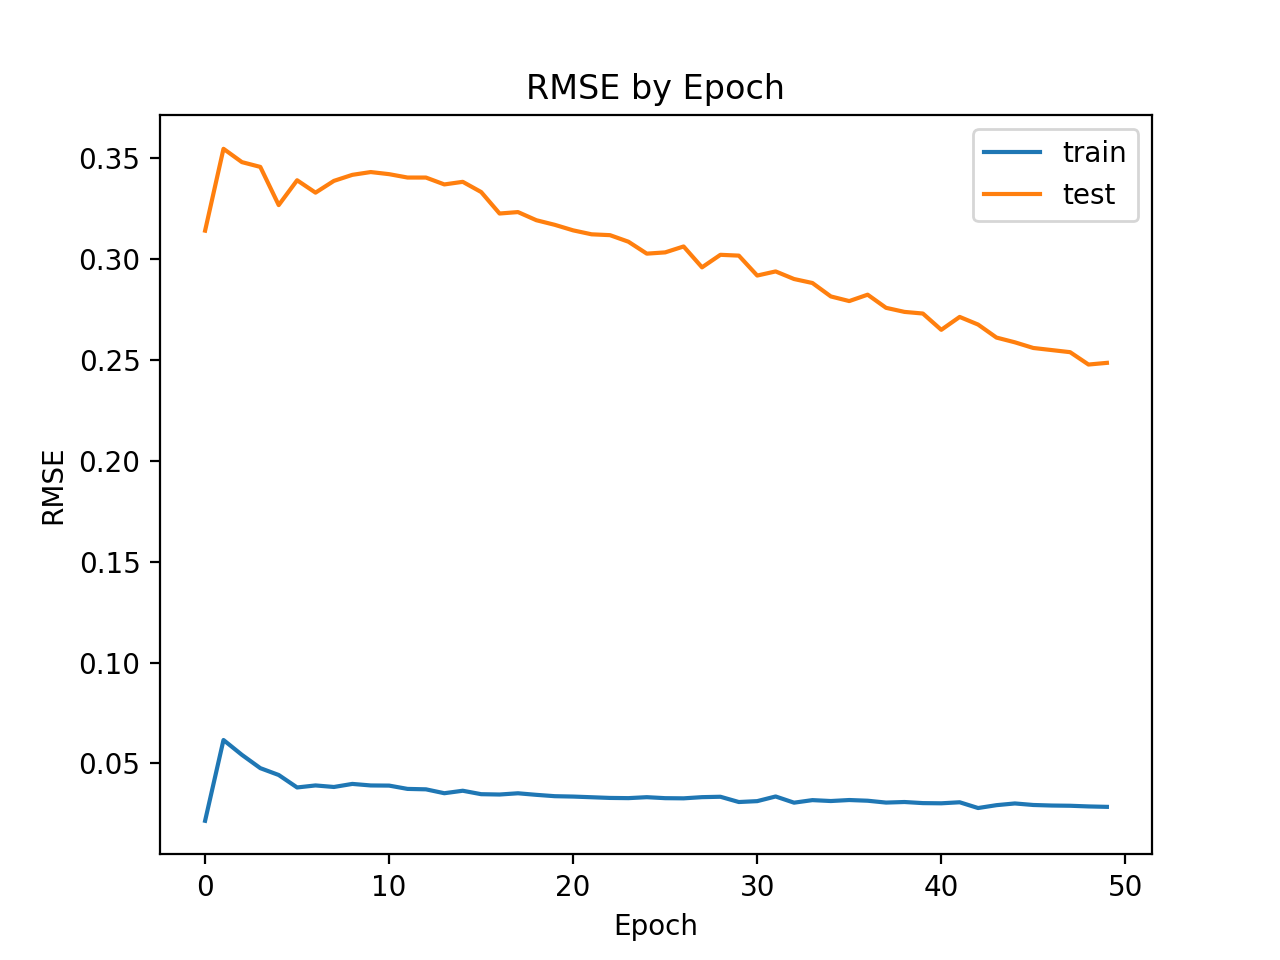
\includegraphics[scale=0.60 ]{../pic/rnn.png}
\end{figure}

After implementing the RNN with LSTM we were still unhappy with our results, ending with an RMSE at 126890.  While the improvement over straight RNN was impressive, the algorithm was still barely better at predicting the price of the future than random, even if it was correctly predicting if the next minute was higher or lower than the previous.  We decided that we needed to make some improvements to the dataset in order to get where we wanted to be. \\

\section{ How It Got Better }

\subsection{ Changing the Model }
We realized our actions were part of a discrete set: buy, sell, or hold. This indicated that a decision tree may also be a viable candidate for our model. Using continuous data features, the decision tree was able to accurately classify each data point with its corresponding action. This was counterintuitive to us. We initially tried it just to test the possibilities, but by tweaking various hyperparameters (such as the percentage split for test/training data, shuffled vs. standard, etc.) the model was able to produce results that seemed almost too good to be true.  \\

\subsection{ Improving the Feature Set }
After changing the algorithm we used, we wanted to see if changing some of the features in our dataset would help as well. Our process for finding new features was to try and think a little outside of the box on what other values out there in the world might have an effect on, or correlation with, Bitcoin prices. One factor that we thought might have a direct effect was the price of Ethereum. Ethereum is one of the leaders in cryptocurrency and it?s value is very strongly connected to bitcoin. We thought that perhaps our algorithms could more successfully predict future bitcoin prices if it knew about Ethereum prices as well. \\

Another data feature that we decided to add into our new dataset was an RSI (relative strength index) value. Luckily, we were able to get a good RSI value from the Neuryx API. The RSI value is a number between 0 and 100 that indicates the momentum of the price graph. If the prices of bitcoin are in a steep down turn, the the RSI value will be closer to 0. Similarly, if the prices are positively spiking, then the RSI will be closer to 100, and if the bitcoin prices are staying around the same value the RSI will be close to 50. We thought that RSI would be a good feature to add to our dataset because it is a good indicator of previous data in itself. Since decision tree algorithms don?t necessarily have a concept of time, this feature could add that factor into our final results. \\

For reference, compare the figure below to the one previously shown concerning the RNN. Notice how the RMSE is drastically reduced.

\begin{figure}[H]
	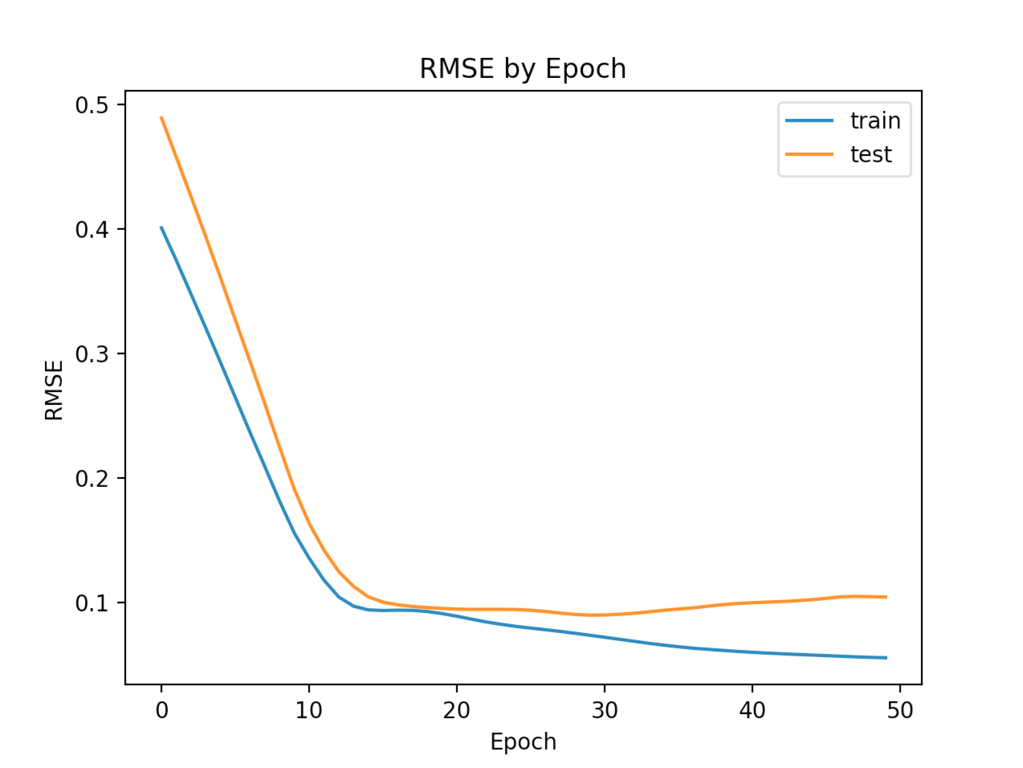
\includegraphics[scale=0.55 ]{../pic/rnn_new.png}
\end{figure}


\section{ Final Results }

When implementing the decision tree, we were very surprised to see initial performance around ~95\% classification accuracy when classifying the currency as any one of three options: Buy, Hold, or Sell. As discussed above, these labels were assigned based on a moving average of the currency's performance over a fixed period of time. This was beyond our optimistic expectations for this model, so we gave it a more robust validation by running it with different test and train splits. It consistently performed with around 95\% accuracy (+-1\%). In the problem domain, the ability to predict Buy, Hold, or Sell accurately even just over 50\% of the time can produce incredible ROIs. So we see these results as encouraging. \\

\begin{figure}[H]
	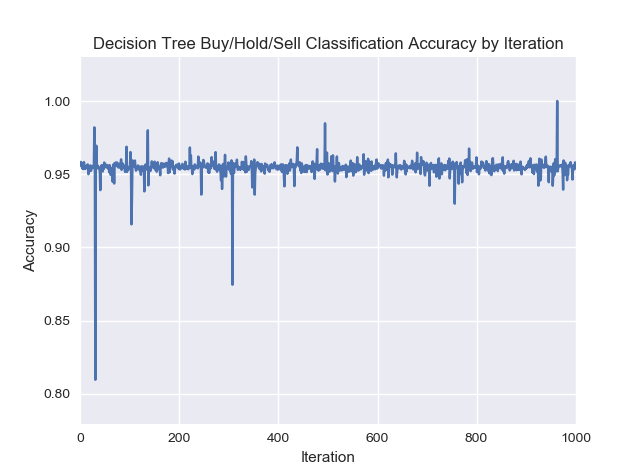
\includegraphics[scale=0.55 ]{../pic/iteration.png}
\end{figure}

Additionally, we found that for most training/test splits of the data, accuracy remained consistent around 95\%. From this we conclude that our decision tree model was able to successfully generalize to novel data. This implied nor only a robust model, but also a model flexible enough to handle the volatility of the market. \\

\begin{figure}[H]
	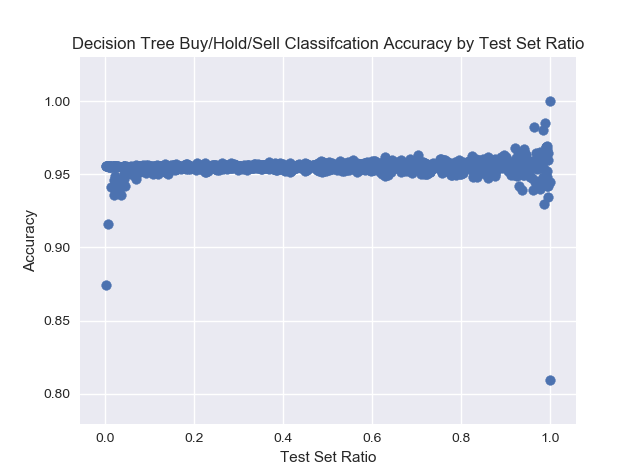
\includegraphics[scale=0.55 ]{../pic/ration.png}
\end{figure}

We also testing the decision tree on several sizes of data, from small subsets to the entire dataset available. Again, the results were surprising (although by this point, nothing could surprise us anymore). The figure below shows that smaller sets have a slightly lower accuracy, while larger sets have slightly higher ones, but overall the average stays right around 95\%. This tells us that the trends the machine is learning are present in the majority of the data points, rather than a flukey streak of luck found in a particular subset. \\

\begin{figure}
	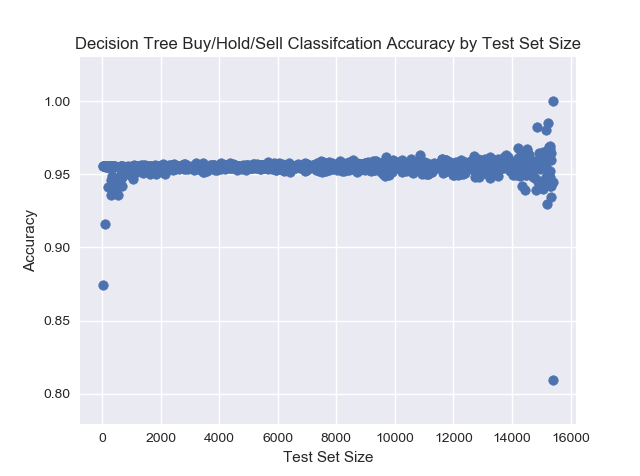
\includegraphics[scale=0.55 ]{../pic/size.png}
\end{figure}

\subsection{ Explanation }

As mentioned, the results seemed too good to be true. Although we were hopeful, we remained skeptical. We tested several variations of data features, hyperparameters, and datasets, but the results persisted. We are left to conclude that we are either a) very lucky, or b) that the model has learned a pattern within the individual data points that determines whether the user should buy, sell, or hold their cryptocurrency. This is especially interesting because it abstracts the data from its time sequence, which we originally thought would be a relevant point. \\

\subsection{ Training \& Testing }
\subsubsection{ RNN }
To train the RNN, we had to first split the dataset into training and testing sets, the network was able to learn the data relatively fast; we ran about 50 epochs. Once trained, we could verify by running the test subset of the data through the machine, recording the results. In order to use this model, we simply run the row of data through the network as the API fetcher returns the row, which immediately (since it is already trained) spits out a user action.\\

\subsubsection{ Decision Tree }
The decision tree was also split into testing and training data. Then, any nominal data needed to be replaced by a numeric substitution. the tree was then trained (with various dataset splits) so that it could be verified by the test set. Similarly to the RNN, the tree can be invoked as rows of data are fetched in order to produce instantaneous results. \\

\section{ Conclusion }
Although the RNN with LSTM made a significant improvement upon the standard RNN, it did not provide predictions much more accurate than a random guess. This was somewhat disappointing, but it was also somewhat expected. People are constantly trying to make market prediction algorithms that have high accuracy because running such an algorithm can make a lot of money. However, it is common knowledge that it is very difficult to successfully predict with higher than 50\% accuracy on these types of problems. Thus, our RNN with LSTM seemed to fit right in with any other mediocre algorithm out there that solves a market value prediction problem such as ours. \\

Upon further study, however, we found a way to sharply increase our accuracy. We found that the Decision Tree consistently performed well beyond both the standard RNN and the RNN with LSTM. But given the time-series nature of our problem, we remain somewhat skeptical as to the reliability of this model alone and believe it needs further validation. Our ideas regarding potential improvements that we would make if time permitted will be discussed in the following section. \\

\subsection{ Moving Forward }
Although both models performed well, we believe there is room for accuracy improvement and model validation. The RNN with LSTM conceptually seems to fit the time series nature of the problem much better than the Decision Tree, yet it underperformed. If time allowed, we would return to the RNN to test other variations. There are many similarities between cryptocurrency price prediction and natural language processing. We would have liked explore further into these domains to assess whether there are any valuable insights to be gained. \\

Additionally, we would like to test our models in more bullish market conditions. The cryptocurrency market has followed a steady downward trend since we selected this project and began gathering data. It would be enlightening to collect data during a particularly active period, or else adjust our model to also trade typical stocks. \\

We would like to test the model's predictive powers with a mock portfolio of cryptocurrencies that bought, sold, and held according to the model?s predictions. This would be the ultimate measurement as to how reliable it is. If it can make money in a mock portfolio, we know that the model is good enough. \\

\subsection{ Feature Refinement }
As previously mentioned, we sought to keep our initial feature set minimal, filtering potential features if we did not see a logical correlation to the short-term bitcoin price. Over the past few months, the major cryptocurrencies have dropped dramatically in value due to unfavorable news cycles and government announcements. These events have had a significant effect on investor sentiment, and consequently on the price of cryptocurrencies. While this information might be embedded within the features we have already selected, it would be interesting to see what insight could be gained by conducting a sentiment analysis from the most recent news articles mentioning a given cryptocurrency and providing that as a feature. We are certain that this is but one of many other possible features that could improve our results.

\subsection{ Key Takeaways }
\subsubsection{ 1. Let the Data Speak for Itself }
There are certain problems within the realm of machine learning that are beyond the comprehension of the human mind. We as humans cannot intuitively understand multi-dimensional data and complex time series. However, if we can understand the models used by computers, the machines can learn the data and present it in a way that we as humans can interpret. Rather than trying to analyze the data points to predict the crypto market, we let the machine run its course and learned data trends we never could have.
\subsubsection{ 2. Try Everything}
Even if you think a model is a poor fit, or a data feature is useless, it may be worth it to try anyway. Machine learning and big data are complex topics that, as stated above, can't be intuitively understood by the human brain. We thought the RNN was a perfect fit, and frankly that a decision tree was a poor fit. However, the results proved the opposite to be true.
\subsubsection{ 3. A model Is Only As Good As Its Data}
We learned this when we ran the same model with different datasets- if the data is poor, so will the results be poor. Spectacular data, however, can produce spectacular results. It is worth the extra effort to choose the right data and clean it up.

\end{document}